\chapter{Type Annotation on Unstructured Texts}
\label{cha:cetus}
\graffito{
This chapter presents CETUS, a pattern-based approach for annotating \ac{RDF} type information to entities.
CETUS has won the OKE challenge 2015~\cite{okechallenge}, task 2, and is published in the corresponding article~\cite{CETUS_2015}.
The author of this thesis assisted the main author in programming, co-wrote the paper~\cite{CETUS_2015} and presented its poster. 
}


Standard document processing pipelines miss the opportunity to gain insights from semantic entities novel to the underlying \ac{KB}. 
That is, most known tool chains recognize entities based on linguistic models and link them to a \ac{KB} or null if they are emerging entities. 
So far, linking novel entities has only been the concern of a few approaches~\cite{AIDA,agdistis_iswc}.
Consequently, extracting type information for emerging and existing entities is a novel research avenue so far only tackled by the TAC KBP \ac{EL} challenge 2014\footnote{\url{http://nlp.cs.rpi.edu/kbp/2014/}}, the Micropost workshop series\footnote{\url{http://www.scc.lancs.ac.uk/microposts2015/}} and the OKE challenge 2015~\cite{okechallenge}.

We present CETUS, a novel pattern based entity type extraction framework for identifying the type of a given entity inside a given text and linking this type to a \ac{KB}, i.e., to the subset of the DOLCE+DnS Ultra Lite ontology classes\footnote{\url{http://www.ontologydesignpatterns.org/ont/dul/DUL.owl}}.
Here the subset refers to \texttt{dul:Person}, \texttt{dul:Place}, \texttt{dul:Organization} and \texttt{dul:Role}.
CETUS' pipeline is divided into three subsequent parts: i) an a-priori pattern extraction, ii) a grammar-based analysis of the input document and iii) a mapping of the type evidence to the DOLCE+DnS Ultra Lite classes. 
Our contributions are as follows:
\begin{itemize}
\item CETUS is a fast and easy to implement baseline approach to path a way to novel research insights.
\item Our approach implements two approaches for the third step using the YAGO ontology as well as the FOX~\cite{FOX} \ac{NER} framework.
\item CETUS outperforms other apprroaches~\cite{okechallenge} w.r.t. the OKE challenge 2015 and thus is able to generate novel \ac{RDF} data from unstructured text.
\end{itemize}

In the following, we will explain these parts in detail.
The open source code of CETUS can be found at \url{https://github.com/AKSW/Cetus}.
\section{Pattern Extraction}
\label{sec:patternExt}

The patterns used for identifying the type of an entity inside a document, are generated semi-automatically in an iterative manner.
First, CETUS identifies phrases containing entities and their types in a given document corpus (here we use the DBpedia 2014 abstracts) and extracts them.
After sorting these phrases according to the string in between the entity and its type, we analyze them and create the patterns in an incremental process.
The progress of our pattern extraction is measured by the amount of phrases that are covered by our patterns.
In the following, these steps are described in more detail.

\subsection{Sentence Part Extraction}

For extracting the phrases containing entities and their types, we used the abstracts of the English DBpedia 2014 abstracts dump file.
Every abstract describes the entity it belongs to and, thus, contains the label of the entity and its type.
We assume, abstracts are written properly and thus contain both information.

First, CETUS preprocesses each abstract individually.
Our approach removes the text written in brackets, e.g., pronunciations.
%Afterwards, we use the Stanford Deterministic Coreference Resolution System~\cite{Lee2013} to replace pronouns with their coreferenced words, e.g., \emph{He studied physics} with \emph{Albert Einstein studied physics}.
Next step of the preprocessing is the splitting of the abstracts into single sentences.
%\todo[inline]{@Micha: still valid?}
Second, sentences containing the entity label and at least one label of one of its types (\texttt{rdf:type}) are processed further.
CETUS extracts the part of the sentence between the entity label and the type label and stores additionally the words, their lemmas and part-of-speech tags of the extracted phrase.

After analysing all abstracts, CETUS counts the different phrases.
The words inside these parts are encoded as \texttt{<word>\_<lemma>\_<pos-tag>}.
Table~\ref{tab:extParts} shows examples of extracted phrases and their counts how often they have been found inside the English DBpedia.

Delving into the extracted phrases reveals insights into the structure of entity type descriptions in DBpedia abstracts.
That is, the formulation "\texttt{<entity>} \emph{is a} \texttt{<type>}" occurs most often.
%The second most common formulation is nearly the only one in our list, in which the type precedes the entity.
The second most common formulation uses a type preceding the entity and is listed as the second example in Table~\ref{tab:extParts}.
The third example is a variant of the first one containing the determine "an" instead of "a".
The fourth example shows that some abstracts contain more complex formulations like "\texttt{<entity>} \emph{is a} \texttt{<type>} \emph{of} \texttt{<type>}" while the last example contains an additional adjective that was not a part of the types label, i.e., "flowering".

\begin{table}[htb!]
\centering
\resizebox{\textwidth}{!}{
\begin{tabular}{lp{5mm}r}
 \toprule
 \multicolumn{1}{c}{\textbf{Extracted phrase}} && \multicolumn{1}{c}{\textbf{Count}} \\
 \midrule
 \texttt{<entity> is\_be\_vbz a\_a\_dt <type>} && 242\,806 \\
 \texttt{<type> <entity>} && 107\,082 \\
 \texttt{<entity> is\_be\_vbz an\_an\_dt <type>} && 12\,981 \\
 \texttt{<entity> is\_be\_vbz a\_a\_dt species\_species\_n1 of\_of\_pp-f <type>} && 12\,554 \\
 \texttt{<entity> is\_be\_vbz a\_a\_dt species\_species\_n1} && \multirow{2}{*}{4\,069} \\ 
 \qquad\qquad\ \ \texttt{of\_of\_pp-f flowering\_flower\_j-vvg <type>} && \\
 \bottomrule
\end{tabular}
}
\caption{Examples of sentence parts found between an entity and its type.}
\label{tab:extParts}
\end{table}

\subsection{Grammar Construction}
\label{sec:grammar}

The aim of creating a grammar is to generate a parser that is able to identify the part of a sentence describing  the type of an entity,
The parser is based on the given position of the entity inside the sentence.
For generating a parser based on our grammar, we are using the ANTLR4 library\footnote{\url{http://www.antlr.org/}}.

Our grammar is based on the following assumptions:
\begin{enumerate}
\item A sentence contains an entity and a type. Otherwise the sentence is not part of our grammar language.
\item A type must contain a noun, but can contain additional words that are specifying the meaning of the noun, e.g., adjectives.
%Note, that the type is not a noun phrase!
\end{enumerate}

The first assumption simplifies the task of defining a grammar since we can focus on the sentences that are important for our task and ignore all others.
The second assumption contains the definition of a type surface form.
It might seem to be contradictory w.r.t. the last example of Table~\ref{tab:extParts} but for the extraction it is important that we extract all words that \emph{could} be part of the types surface form.
Following this assumptions, we can define a type inside the grammar with the rule in Listing~\ref{lst:typeRule}.

\lstset{
%  basicstyle=\footnotesize\ttfamily,
%  breaklines=true,
%  captionpos=b,                    % sets the caption-position to bottom
%  frame=single,
%  %morecomment=[s][\color{blue}]{<}{>},
%  morecomment=[s][\color{red}]{"}{"},
  numbers=none
%  
%%  numbersep=5pt,
%% numberstyle=\tiny,
%%  stringstyle=\tiny
}

\begin{figure}[htb!]
\begin{lstlisting}[label=lst:typeRule, caption=The grammar rule defining a type surface form.]{typeRule}
type : (ADJECTIVE|VERB|ADVERB)* FOREIGN? NOUN+;
\end{lstlisting}
\end{figure}

A surface form of a type can contain a number of adjectives, verbs or adverbs as well as a foreign word, e.g., the latin word "sub".
Additionally, a type has one or more nouns.

As mentioned above, the construction of the grammar is designed to be an iterative, incremental, self-improving process.
We start with the simple \emph{is-a} pattern that matches the most common phrase "\texttt{<entity>} \emph{is a} \texttt{<type>}". 
The definition of this pattern is shown in Listing~\ref{lst:firstIsARule}.
\begin{figure}[htb!]
\begin{lstlisting}[label=lst:firstIsARule,caption=First simple version of the \emph{is-a} pattern. \texttt{ENTITY} marks the position of an entity.]{firstIsARule}
is_a_pattern : ENTITY is_is_vbz a_a_dt type;
\end{lstlisting}
\end{figure}

With this simple grammar, we try to match all phrases extracted beforehand and create a list containing all those phrases that have not been matched so far.
Using this list, we extend our grammar to match other phrases.
In our example, we extend the simple \emph{is-a} pattern towards matching different temporal forms of the verb "be" and different determiners, e.g., "a" and "an", see Listing~\ref{lst:secondIsARule}.


\begin{figure}[htb!]
\begin{lstlisting}[label=lst:secondIsARule,caption=Extended version of the \emph{is-a} pattern.]{secondIsARule}
is_a_pattern : ENTITY FORM_OF_BE DETERMINER <type>

FORM_OF_BE : ~[ \t\r\n]+ '_be_v' ~[ \t\r\n]*;
DETERMINER : ~[ \t\r\n]+ '_' ~[ \t\r\n]+ '_d' ~[ \t\r\n]*;
\end{lstlisting}
\end{figure}

With this iterative, incremental process, we further extended the grammar until we covered more than 90\% of the extracted phrases.
The complete grammar can be found in the projects source code repository.

%\subsection{Example Patterns}

%\todo[inline]{Should we keep this section or delete it?}

%\begin{figure}
%\begin{lstlisting}[label=lst:allPatternRules,caption=The grammar rules for finding a type surface form.]{allPatternRules}
%sentence : WORD* ENTITY (COMMA (WORD|POINT|COMMA|COLON)+ COMMA)? type_after_entity_pattern (WORD|POINT|COMMA|COLON)*
%| WORD* type_in_front_of_entity ENTITY WORD*;
%
%type_after_entity_pattern : is_a_type_of_pattern
%| is_a_pattern
%| type_with_dt ;
%
%is_a_pattern : FORM_OF_BE type_with_dt (((COMMA? AND) | COMMA) type_with_dt)*;
%is_a_type_of_pattern : FORM_OF_BE type_with_dt OF type_with_dt;
%
%type_in_front_of_entity : type_with_dt (OF|COMMA|COLON)?;
%
%type_with_dt : DETERMINER? nr_or_crd? type;
%nr_or_crd : NUMBER | CARDINAL_NUMBER;
%\end{lstlisting}
%\end{figure}

\section{Type Extraction}
\label{sec:docAnalysis}

The pattern-based type extraction can be separated into two steps.
The first step extracts type evidence strings from the text, while the second step creates a local type hierarchy based on the extracted string.
Following, we describe both steps in more detail.

\subsection{Type String Extraction}

To identify the type evidence string for a certain entity, CETUS extracts the string containing the type of a given entity from a given text using the grammar from above.
Let us assume the following running example: 

\begin{center}
\emph{\textbf{Albert Einstein} was a German-born theoretical physicist. In 1921, he got the Nobel Prize in Physics. }
\end{center}

CETUS processes the document as input with "Albert Einstein" marked as entity.
The text is split into sentences and the surface form of the entity is replaced by a placeholder. 

\begin{center}
\emph{\textbf{ENTITY} was a German-born theoretical physicist.}

\emph{In 1921, he got the Nobel Prize in Physics.}
\end{center}

A parser based on the grammar from Section~\ref{sec:grammar} is applied to every sentence.
While the second sentence is identified as not contained in the language of the grammar, the first sentence is identified to be in the language.
Here, we discard the second sentence from further processing, although a co-reference resolution~\cite{NgongaNgomo2014} approach could increase the performance in other cases.
Moreover, the parser identifies "German-born theoretical physicist" as evidence type string.

\subsection{Local Type Hierarchy}

Based on the extracted evidence type string, CETUS creates a type hierarchy and links the given entity to the hierarchy.
The type hierarchy comprises classes that are generated automatically from the extracted string based on the second assumption of Section~\ref{sec:grammar}.
Each class is generated by concatenating the words found in the extracted string using camel case.
After a class has been created, the first word is removed and the next class is created.
Every following class is a super class of the classes generated before.
Finally, the entity is connected to all generated classes.

For our example, three classes would be generated and linked to the entity as shown in Listing~\ref{lst:localHierarchy} respectivly Figure~\ref{fig:localHierarchy}.%\footnote{The prefix \texttt{ex} could stand for every user defined vocabulary, e.g., \url{http://example.com/}.}.

\begin{figure}[htb!]
\centering
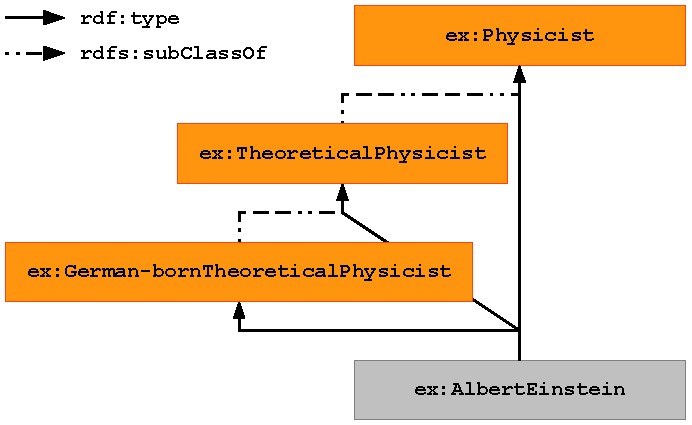
\includegraphics[scale=0.75]{part_02/unstructured_annotation/fig/localHierarchy.pdf}
\caption{Schema of the generated local hierarchy of the example.}
\label{fig:localHierarchy}
\end{figure}

\begin{figure}[htb!]
\begin{lstlisting}[label=lst:localHierarchy,caption=The local hierarchy is generated from the extracted string expressed using Turtle as \ac{RDF} serialization.]{localHierarchy}
ex:AlbertEinstein
    a ex:German-bornTheoreticalPhysicist, 
        ex:TheoreticalPhysicist, ex:Physicist .

ex:German-bornTheoreticalPhysicist
    a rdfs:Class ;
    rdfs:subClassOf ex:TheoreticalPhysicist ;
    rdfs:label "German-born theoretical physicist" .

ex:German-TheoreticalPhysicist
    a rdfs:Class ;
    rdfs:subClassOf ex:Physicist ;
    rdfs:label "theoretical physicist" .

ex:German-Physicist
    a rdfs:Class ;
    rdfs:label "physicist" .

\end{lstlisting}
\end{figure}

\section{Entity Type Linking using YAGO}
\label{sec:linkingyago}

%CETUS approach to link the evidence string to the DOLCE+DnS Ultra Lite classes \texttt{dul:Person}, \texttt{dul:Place}, \texttt{dul:Organization} and \texttt{dul:Role} is twofold.

The linking of the generated classes to a \ac{KB} can be done in two different ways.
Our first approach, CETUS$_{YAGO}$,  uses the labels of the automatically generated classes to find a matching class inside another, well-known \ac{KB}.
CETUS uses the YAGO ontology~\cite{mahdisoltani2014yago3} which comprises a large class hierarchy and, thus, increases the chance to match one of these classes.
YAGO itself contains more than 10 mio. entities and exceeds 350.000 classes.
Our second approach serves as a baseline to our own approach and uses the FOX~\cite{FOX} framework.

First, we created an index containing the surface forms of the YAGO classes with a mapping to the class URIs.
Second, CETUS needs to match every generated class using the approach from Section~\ref{sec:docAnalysis} to one of the labels of the YAGO classes.

Currently, our approach uses 3-gram string similarity to match labels in the index with those of the generated classes as it has been proven to be efficient and effective for such a task~\cite{agdistis_iswc}.
This process retrieves most similar YAGO class for every generated class and a similarity score.
From these YAGO classes, CETUS chooses the class with the highest similarity score.
If two classes have the same score, CETUS chooses the class which is lower inside the local generated type hierarchy.
The chosen YAGO class is linked to its local class.

After that, we iterate through the YAGO class hierarchy from the linked class to its root, searching for one of the classes listed in Table~\ref{tab:yagoClassMatching}.
If such a class is found, we link it with the corresponding DOLCE+DnS Ultra Lite class.
Otherwise, we repeat the search using the YAGO class with the second highest similarity score.
The result for our running example can be seen in Figure~\ref{fig:localYAGOHierarchy}
\begin{table}[htb!]
\centering
\begin{tabular}{lp{5mm}l}
\toprule
 \multicolumn{1}{c}{YAGO class} && DOLCE+DnS Ultra Lite class \\
\midrule
 \texttt{yago:wordnet\_person\_100007846} && \texttt{dul:Person} \\
 \texttt{yago:wordnet\_location\_100027167} && \texttt{dul:Place} \\
 \texttt{yago:wordnet\_organization\_108008335} && \texttt{dul:Organization} \\
 \texttt{yago:wordnet\_role\_100722061} && \texttt{dul:Role} \\
\bottomrule
\end{tabular}
\caption{Mapping from YAGO to DOLCE+DnS Ultra Lite classes.}
\label{tab:yagoClassMatching}
\end{table}

\begin{figure}[htb!]
\centering
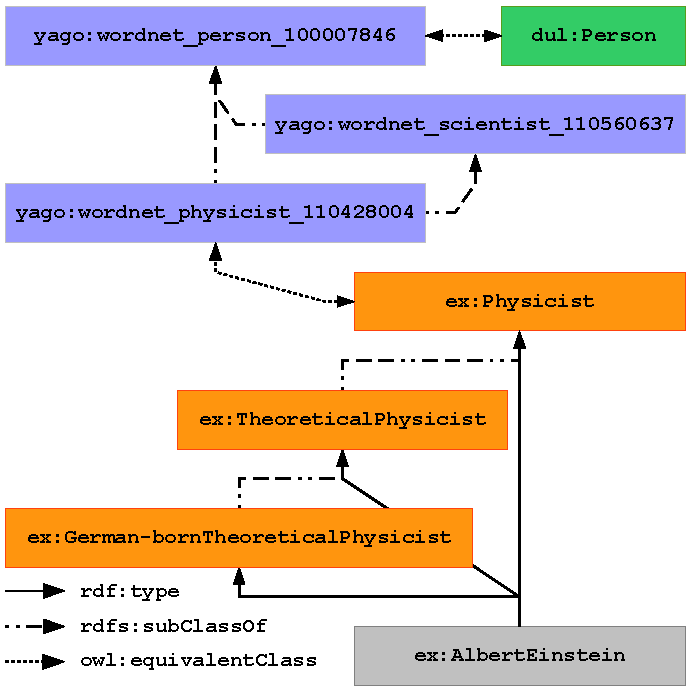
\includegraphics[scale=0.75]{part_02/unstructured_annotation/fig/localYAGOHierarchy.pdf}
\caption{Resulting type hierarchy that is created based on the YAGO ontology.}
\label{fig:localYAGOHierarchy}
\end{figure}

%\begin{table}
%\centering
%\begin{tabular}{@{}ll@{}}
%\toprule
%\textbf{Similarity} & \textbf{Formula/Explanation} \\ \midrule
%Dice-Coefficient Similarity &         \\
%Levenstein/Edit Similarity &         \\
%Euclidean Similarity &         \\ 
%Semantic Similarity &      Word2Vec   \\\bottomrule
%\end{tabular}
%\caption{Similarity measures of CETUS}
%\label{tab:stringsim}
%\end{table}

%CETUS' algorithms are easily extensible via its interfaces. 
%We will refine the set of string matching algorithms after the evaluation against the Open Knowledge Extraction task 2 corpora.



\begin{figure}[htb!]
\centering
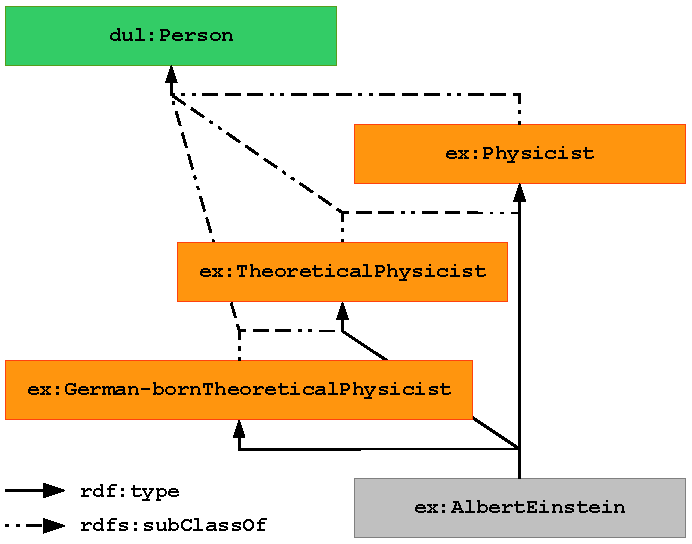
\includegraphics[scale=0.75]{part_02/unstructured_annotation/fig/localFOXHierarchy.pdf}
\caption{Resulting type hierarchy that is created based on the results of FOX.}
\label{fig:localFOXHierarchy}
\end{figure}
\section{Entity Type Linking using FOX}
\label{sec:typeLinking}
A second approach for a type extraction baseline is the usage of one of the various, existing entity typing frameworks.
For our second version CETUS$_{FOX}$, we are using FOX, a \ac{NER} and typing framewrok based on ensemble learning over 8 different tools.

\begin{table}
\centering
\begin{tabular}{lp{5mm}l}
\toprule
 \multicolumn{1}{c}{FOX class} && DOLCE+DnS Ultra Lite class \\
\midrule
 \texttt{scmsann:PERSON} && \texttt{dul:Person} \\
 \texttt{scmsann:LOCATION} && \texttt{dul:Place} \\
 \texttt{scmsann:ORGANIZATION} && \texttt{dul:Organization} \\
 %\texttt{scmsann:OTHER} && \texttt{dul:Role} \\
\bottomrule
\end{tabular}
\caption{Mapping from FOX classes to DOLCE+DnS Ultra Lite classes.}
\label{tab:foxclassmatching}
\end{table}

CETUS$_{FOX}$ sends the given document to the FOX Web service for retrieving annotations.
If the entity inside the document is found and typed by FOX, the type is used to choose one of the four DOLCE+DnS Ultra Lite classes, see Table~\ref{tab:foxclassmatching}.
The chosen class is used as super class for the automatically created classes.
Unfortunately, FOX does not identify roles in its current version.

With respect to our running example, FOX marks "Albert Einstein" as a person.
Thus, the created classes would be defined as subclasses of \texttt{dul:Person} as shown in Figure~\ref{fig:localFOXHierarchy}.


